%======================================================================
% CHƯƠNG X: ĐÁNH GIÁ MÔ HÌNH VÀ ỨNG DỤNG TRONG CHẤM ĐIỂM TRẮC NGHIỆM
% (Thay X bằng số thứ tự chương của bạn)
%======================================================================
\chapter{Đánh giá mô hình và ứng dụng trong chấm điểm trắc nghiệm}
\label{chap:danh_gia_ung_dung}

Chương này tập trung vào việc đánh giá hiệu năng của mô hình nhận diện đã xây dựng và trình bày cách thức ứng dụng mô hình này vào một hệ thống chấm điểm trắc nghiệm tự động hoàn chỉnh. Quá trình đánh giá được thực hiện trên một tập dữ liệu độc lập, và các kết quả sẽ được phân tích chi tiết thông qua các độ đo định lượng và trực quan hóa.

\section{Đánh giá hiệu năng mô hình nhận diện}
\label{sec:danh_gia_mo_hinh}
Để đảm bảo tính khách quan và độ tin cậy, mô hình nhận diện các ô tròn được đánh giá trên một bộ dữ liệu kiểm thử mới, được chuẩn bị và gán nhãn độc lập.

\subsection{Tập dữ liệu đánh giá chuyên biệt}
\label{ssec:bo_du_lieu_danh_gia}
Một tập dữ liệu đánh giá chuyên biệt đã được xây dựng nhằm kiểm tra khả năng tổng quát hóa của mô hình. Tập dữ liệu này bao gồm 50 phiếu bài làm trắc nghiệm thực tế, được quét và xử lý. Từ 50 phiếu này, các vùng chứa đối tượng quan tâm (ô tròn) được trích xuất:
\begin{itemize}
    \item \textbf{Phần 1 (Part 1):} Bao gồm 200 ảnh con, được cắt từ vùng chứa các lựa chọn đáp án bài làm phần 1 của thí sinh trên các phiếu.
    \item \textbf{Phần 2 (Part 2):} Bao gồm 200 ảnh con, được cắt từ vùng chứa các lựa chọn đáp án bài làm phần 2 của thí sinh trên các phiếu.
\end{itemize}
Toàn bộ 400 ảnh con này đã được tải lên nền tảng Roboflow để thực hiện việc gán nhãn (annotation) một cách chính xác, tạo ra dữ liệu gốc (ground truth) cho quá trình đánh giá. Mỗi ô tròn trong ảnh con được định vị bằng một hộp giới hạn (bounding box) và gán nhãn tương ứng 
\subsection{Các độ đo đánh giá}
\label{ssec:metrics_danh_gia}
Hiệu năng của mô hình nhận diện được lượng hóa thông qua các độ đo tiêu chuẩn trong bài toán phát hiện đối tượng (object detection):
\begin{itemize}
    \item \textbf{Precision (độ chính xác):} Tỷ lệ các đối tượng được mô hình dự đoán là tích cực (positive) mà thực sự là tích cực.
    \begin{equation}
        \text{Precision} = \frac{TP}{TP + FP}
    \end{equation}
    Trong đó $TP$ (True Positives) là số đối tượng được phát hiện đúng, và $FP$ (False Positives) là số đối tượng bị phát hiện nhầm.
    \item \textbf{Recall (độ phủ):} Tỷ lệ các đối tượng tích cực trong thực tế mà được mô hình phát hiện đúng.
    \begin{equation}
        \text{Recall} = \frac{TP}{TP + FN}
    \end{equation}
    Trong đó $FN$ (False Negatives) là số đối tượng không được phát hiện.
    \item \textbf{F1-score:} Trung bình điều hòa của Precision và Recall, cung cấp một thước đo cân bằng giữa hai chỉ số này.
    \begin{equation}
        F_1 = 2 \times \frac{\text{Precision} \times \text{Recall}}{\text{Precision} + \text{Recall}}
    \end{equation}

    \item \textbf{Confusion Matrix (ma trận nhầm lẫn):} Cung cấp một cái nhìn chi tiết về hiệu suất của mô hình bằng cách hiển thị số lượng dự đoán đúng và sai cho từng lớp đối tượng.
    \item \textbf{Biểu đồ phân bố confidence score:} Phân tích sự phân bố của điểm tin cậy (confidence score) cho các dự đoán, giúp xác định ngưỡng tin cậy phù hợp và hiểu rõ hơn về "sự tự tin" của mô hình.
\end{itemize}
%------------
\section{Kết quả đánh giá định lượng}
\label{ssec:ket_qua_dinh_luong}

Sau quá trình huấn luyện và tối ưu, hiệu năng của mô hình được xác định một cách khách quan thông qua đánh giá trên hai phần của tập dữ liệu thử nghiệm.

\subsection{Đánh giá trên phần 1 của tập dữ liệu}
\label{ssec:ket_qua_phan_1}

Phần 1 của tập dữ liệu được sử dụng để đánh giá ban đầu. Các kết quả định lượng chi tiết, bao gồm các độ đo Precision, Recall, và F1-Score, được tổng hợp trong Bảng \ref{tab:detection_results_part1}.
\begin{table}[H]
    \centering
    \caption{Kết quả đánh giá hiệu năng mô hình trên Phần 1 tập dữ liệu (Lớp ``1'' là ô không tô).}
    \label{tab:detection_results_part1}
    \begin{tabular}{@{}lc@{}}
        \toprule
        Độ đo đánh giá            & Giá trị        \\
        \midrule
        % Dữ liệu từ CM có TP_1=1878, TP_0=630
        % Lớp 1: TP=1878, FP=8(từ 0)+23(từ BG)=31, FN=44(tới 0)+0(tới BG)=44
        Precision (cho lớp 1) & 98.38\%  \\
        Recall (cho lớp 1)    & 97.71\%  \\
        F1-Score (cho lớp 1)  & 98.04\%  \\
        \midrule
        % Lớp 0: TP=630, FP=44(từ 1)+21(từ BG)=65, FN=8(tới 1)+0(tới BG)=8
        Precision (cho lớp 0) & 90.65\%  \\
        Recall (cho lớp 0)    & 98.75\%  \\
        F1-Score (cho lớp 0)  & 94.51\%  \\
        \midrule
        mAP@0.5 (ước tính) & \textasciitilde96-97\% \\
        \bottomrule
    \end{tabular}
\end{table}
Trên Phần 1, mô hình duy trì hiệu suất tốt cho lớp ``1'' (ô không tô). Tuy nhiên, đối với lớp ``0'' (ô tô), chỉ số Precision có phần suy giảm (90.65\%), trong khi Recall vẫn ở mức cao. Điều này cho thấy có sự gia tăng False Positives cho lớp ``0'' trong phần dữ liệu này.

Ma trận nhầm lẫn cho phần 1 (Hình \ref{fig:confusion_matrix_part1}) làm rõ hơn các điểm này.
\begin{figure}[H]
    \centering
    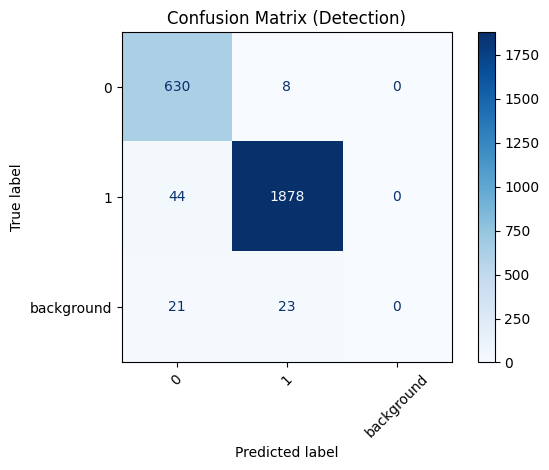
\includegraphics[width=0.75\textwidth]{img_proj/confusionp1.png} % Hình CM của Phần 1 (trước là Part 2)
    \caption{Ma trận nhầm lẫn của mô hình trên phần 1 tập dữ liệu.}
    \label{fig:confusion_matrix_part1}
\end{figure}
Mô hình nhận diện đúng 630 trường hợp cho lớp ``0'' và 1878 trường hợp cho lớp ``1''. Số lượng nhầm lẫn giữa lớp ``0'' và lớp ``1'' vẫn ở mức chấp nhận được. Đáng chú ý, số lượng False Positives từ việc nhầm lẫn nền (background) thành đối tượng tăng lên (21 cho lớp ``0'' và 23 cho lớp ``1''), góp phần làm giảm Precision của lớp ``0''. Không có đối tượng nào bị bỏ sót và phân loại nhầm thành nền.

Phân bố điểm tin cậy trên Phần 1 (Hình \ref{fig:confidence_score_distribution_part1}) cho thấy đa số các phát hiện vẫn có điểm tin cậy cao.
\begin{figure}[H]
    \centering
    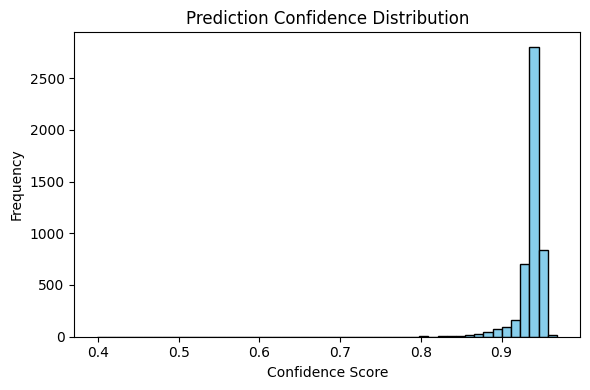
\includegraphics[width=0.75\textwidth]{img_proj/confidencep1.png} % Hình Confidence của Phần 1 (trước là Part 2)
    \caption{Phân bố điểm tin cậy trên Phần 1 tập dữ liệu.}
    \label{fig:confidence_score_distribution_part1}
\end{figure}
Đa số các phát hiện vẫn có điểm tin cậy cao, tập trung quanh 0.9-0.95, thể hiện sự tự tin của mô hình.

Ảnh hưởng của ngưỡng tin cậy trên phần 1 (hình \ref{fig:metrics_vs_threshold_part1}) cho thấy một số đặc điểm.
\begin{figure}[H]
    \centering
    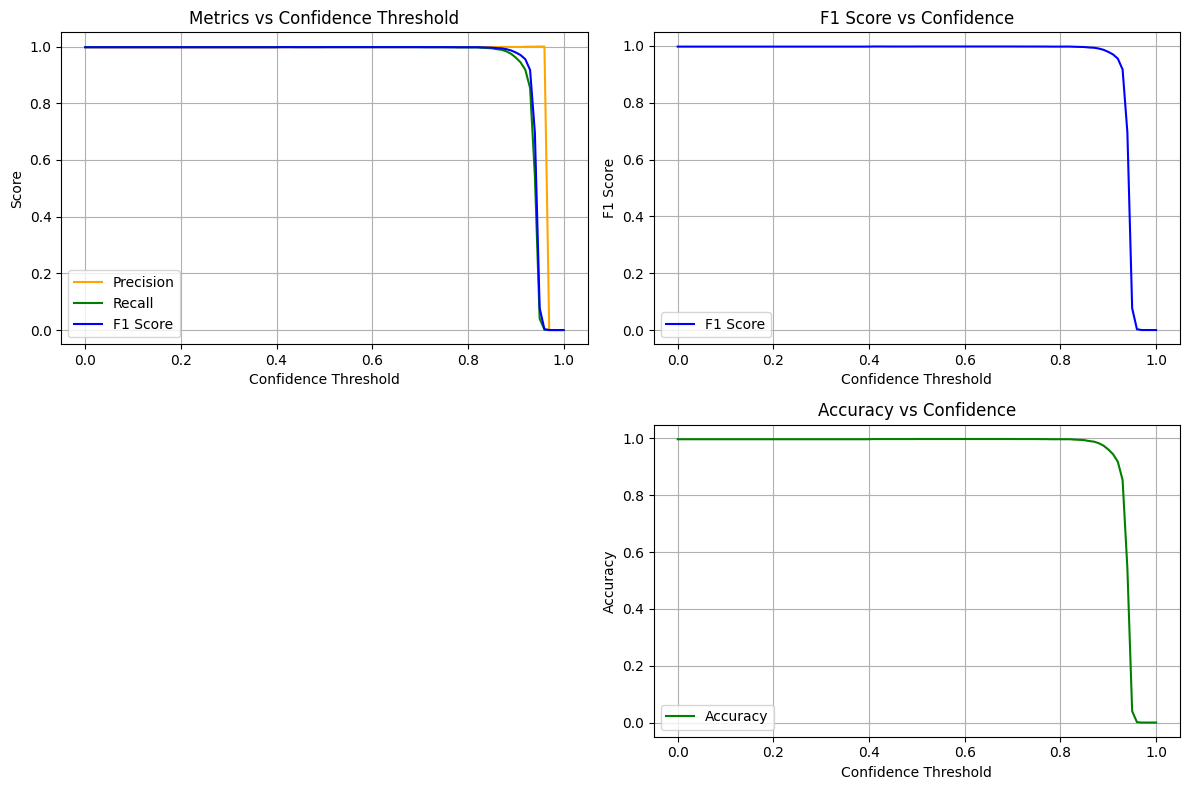
\includegraphics[width=0.9\textwidth]{img_proj/metricp1.png} % Hình Metrics của Phần 1 (trước là Part 2)
    \caption{Ảnh hưởng của ngưỡng tin cậy lên hiệu năng trên phần 1 tập dữ liệu.}
    \label{fig:metrics_vs_threshold_part1}
\end{figure}
Các độ đo Precision, Recall, F1-score và Accuracy vẫn duy trì ở mức cao. Tuy nhiên, sự suy giảm của Recall và F1-Score bắt đầu rõ rệt hơn khi ngưỡng tin cậy vượt quá khoảng 0.8. Precision duy trì ở mức cao cho đến ngưỡng gần 0.85. Điều này gợi ý rằng việc lựa chọn ngưỡng tối ưu cho phần 1 có thể cần cân nhắc kỹ hơn để duy trì Recall mong muốn.

\subsection{Đánh giá trên phần 2 của tập dữ liệu}
\label{ssec:ket_qua_phan_2}

Mô hình tiếp tục được đánh giá trên phần 2 của tập dữ liệu để kiểm tra tính nhất quán về hiệu năng. Kết quả được trình bày trong Bảng \ref{tab:detection_results_part2}.
\begin{table}[H]
    \centering
    \caption{Kết quả đánh giá hiệu năng mô hình trên Phần 2 tập dữ liệu (Lớp ``1'' giả định là ô không tô).}
    \label{tab:detection_results_part2}
    \begin{tabular}{@{}lc@{}}
        \toprule
        Độ đo đánh giá            & Giá trị        \\
        \midrule
        % Dữ liệu từ CM có TP_1=2417, TP_0=2373
        Precision (cho lớp 1) & 99.83\%  \\
        Recall (cho lớp 1)    & 99.71\%  \\
        F1-Score (cho lớp 1)  & 99.77\%  \\
        \midrule
        Precision (cho Lớp 0) & 99.54\%  \\
        Recall (cho Lớp 0)    & 99.87\%  \\
        F1-Score (cho Lớp 0)  & 99.70\%  \\
        \midrule
        mAP@0.5 (ước tính) & \textasciitilde99\% \\
        \bottomrule
    \end{tabular}
\end{table}
Trên Phần 2, các chỉ số trong bảng \ref{tab:detection_results_part2} đều đạt giá trị rất cao, phản ánh khả năng nhận diện chính xác và đầy đủ các đối tượng mục tiêu trong phần dữ liệu này.

Ma trận nhầm lẫn (hình \ref{fig:confusion_matrix_part2}) cung cấp cái nhìn chi tiết về hiệu suất phân loại vượt trội.
\begin{figure}[H]
    \centering
    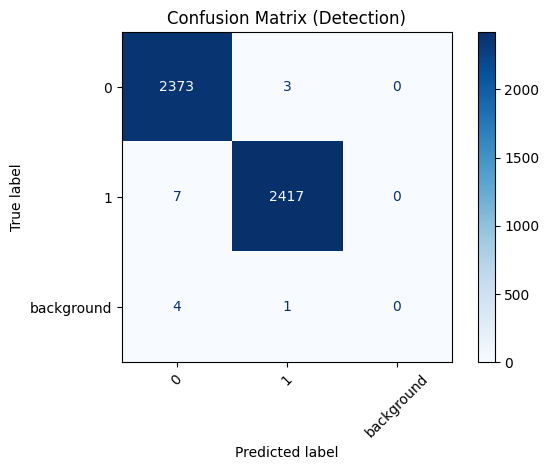
\includegraphics[width=0.75\textwidth]{img_proj/danggiap2.png} % Hình CM của Phần 2 (trước là Part 1)
    \caption{Ma trận nhầm lẫn của mô hình trên phần 2 tập dữ liệu.}
    \label{fig:confusion_matrix_part2}
\end{figure}
Quan sát ma trận, mô hình cho thấy khả năng phân loại xuất sắc giữa lớp ``0'' (2373 dự đoán đúng) và lớp ``1'' (2417 dự đoán đúng). Số lượng nhầm lẫn giữa hai lớp này là không đáng kể. Tỷ lệ False Positive do nhầm lẫn nền (background) thành đối tượng cũng ở mức rất thấp (tổng cộng 5 trường hợp). Đặc biệt, không có đối tượng nào bị bỏ sót và phân loại nhầm thành nền.

Phân bố điểm tin cậy của các phát hiện trên phần 2 (hình \ref{fig:confidence_score_distribution_part2}) củng cố thêm độ tin cậy cao của mô hình.
\begin{figure}[H]
    \centering
    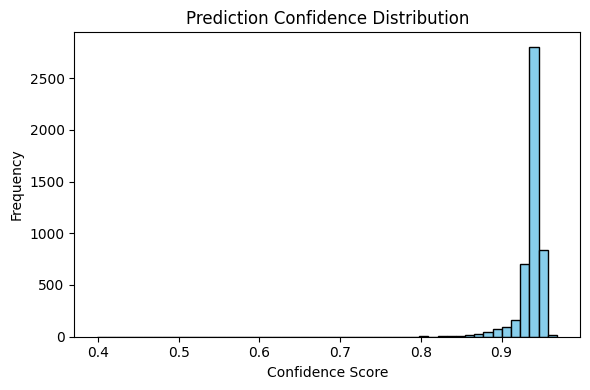
\includegraphics[width=0.75\textwidth]{img_proj/confidence.png} % Hình Confidence của Phần 2 (trước là Part 1)
    \caption{Phân bố điểm tin cậy trên phần 2 tập dữ liệu.}
    \label{fig:confidence_score_distribution_part2}
\end{figure}
Phần lớn các đối tượng được phát hiện có điểm tin cậy rất cao, tập trung ở khoảng 0.9 đến 0.95, cho thấy sự tự tin cao của mô hình vào các dự đoán.

Mối quan hệ giữa ngưỡng tin cậy và các độ đo hiệu năng (hình \ref{fig:metrics_vs_threshold_part2}) cho thấy sự ổn định của mô hình trên phần 2.
\begin{figure}[H]
    \centering
    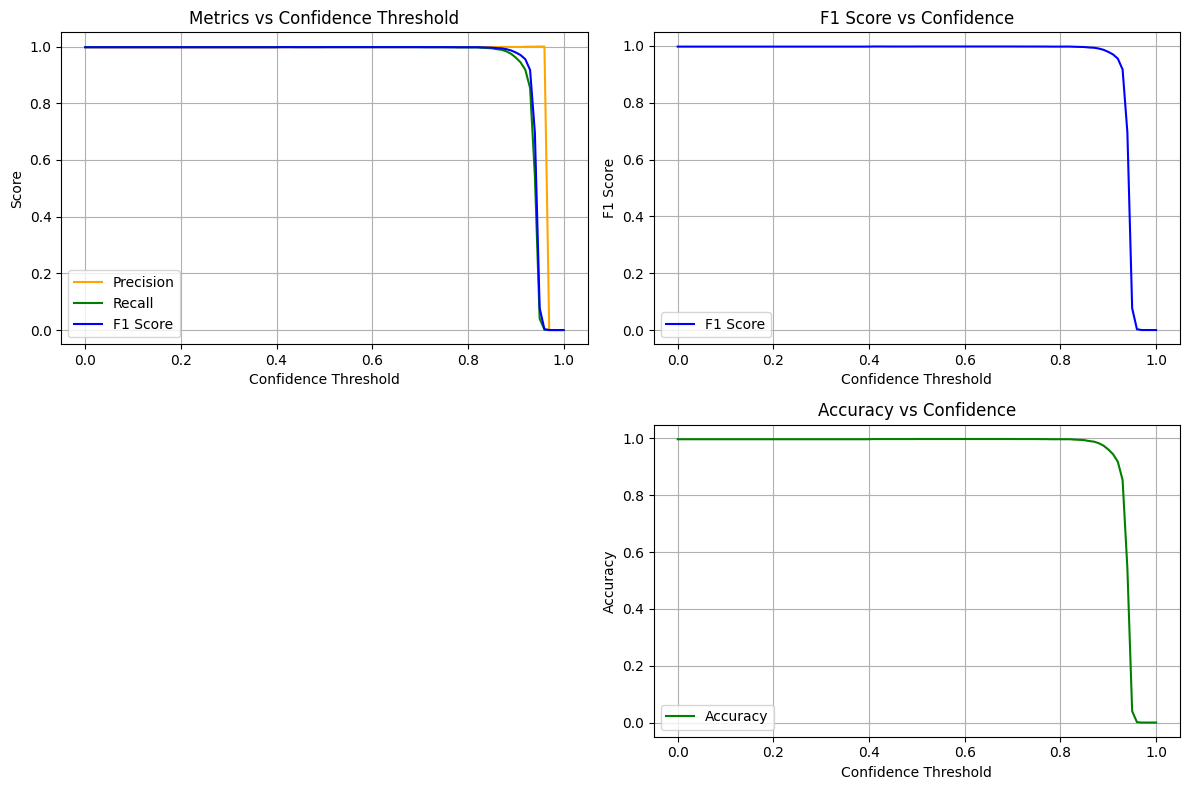
\includegraphics[width=0.9\textwidth]{img_proj/metrix.png} % Hình Metrics của Phần 2 (trước là Part 1)
    \caption{Ảnh hưởng của ngưỡng tin cậy lên hiệu năng trên phần 2 tập dữ liệu.}
    \label{fig:metrics_vs_threshold_part2}
\end{figure}
Các độ đo Precision, Recall, F1-Score và Accuracy duy trì ở mức cao (gần 1.0) cho đến ngưỡng tin cậy khoảng 0.85. Vượt qua ngưỡng này, các chỉ số, đặc biệt là Recall và F1-Score, bắt đầu suy giảm do việc loại bỏ các dự đoán đúng có độ tin cậy thấp hơn. Sự ổn định này ngụ ý mô hình không quá nhạy cảm với việc lựa chọn ngưỡng, và một ngưỡng trong khoảng 0.5 đến 0.85 có thể cân bằng tốt giữa Precision và Recall.

\subsection{Nhận xét chung}
Tổng hợp kết quả từ cả hai phần đánh giá, mô hình phát triển thể hiện hiệu suất mạnh mẽ và đáng tin cậy. Phần 2 của tập dữ liệu cho thấy hiệu năng gần như hoàn hảo, trong khi phần 1, mặc dù có sự suy giảm nhẹ ở Precision của một lớp, vẫn duy trì được khả năng nhận diện tốt. Phân bố điểm tin cậy cao và sự ổn định tương đối của các độ đo theo ngưỡng tin cậy là những dấu hiệu tích cực về độ tin cậy và tính ứng dụng của mô hình. Sự khác biệt nhỏ về hiệu năng giữa hai phần dữ liệu có thể gợi ý về sự đa dạng trong đặc điểm của các ảnh hoặc đối tượng, và có thể được xem xét để cải tiến mô hình hơn nữa trong tương lai.
%------------
\section{Phân tích kết quả nhận diện trực quan}
\label{sec:ket_qua_nhan_dien_truc_quan}

Việc kiểm tra trực quan các kết quả nhận diện bổ sung cho các đánh giá định lượng, giúp hiểu rõ hơn về hành vi của mô hình. Hình \ref{fig:qualitative_detection_examples} trình bày một số ví dụ minh họa. Các ô được mô hình xác định là "được tô" (đáp án chọn) được đánh dấu bằng khung màu đỏ, và các ô "không được tô" có khung màu xanh.

\begin{figure}[H]
    \centering
    \begin{subfigure}[b]{0.48\textwidth}
        \centering
        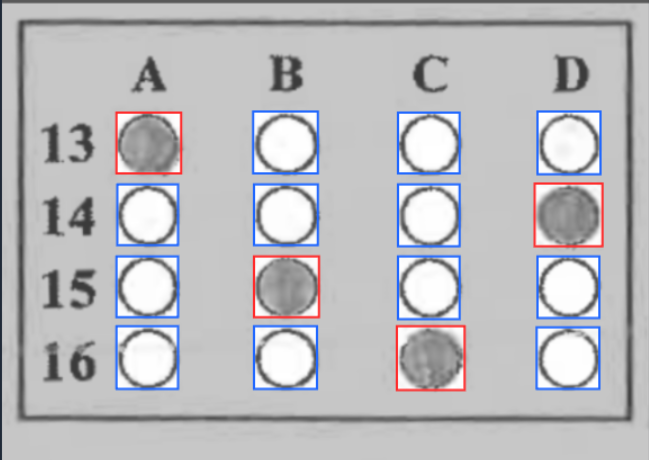
\includegraphics[width=0.85\textwidth]{img_proj/tp1.png}
        \caption{Nhận diện trên phần 1, tô chuẩn.}
        \label{fig:detection_part1_standard}
    \end{subfigure}
    \hfill
    \begin{subfigure}[b]{0.48\textwidth}
        \centering
        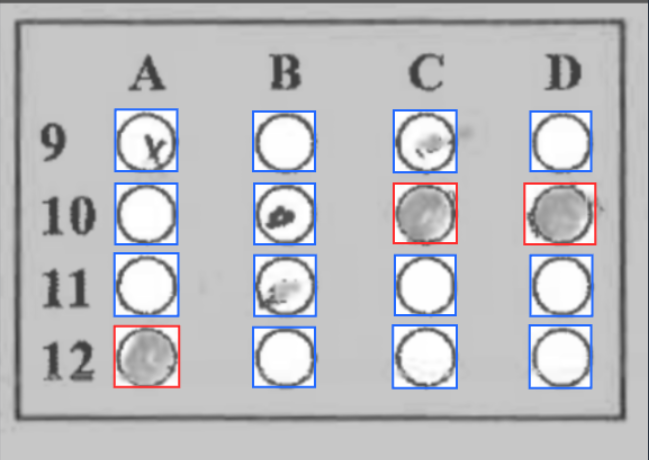
\includegraphics[width=0.85\textwidth]{img_proj/tp11.png}
        \caption{Nhận diện trên phần 1, tô lem nhem.}
        \label{fig:detection_part1_messy}
    \end{subfigure}
    
    \vspace{0.5cm}
    
    \begin{subfigure}[b]{0.48\textwidth}
        \centering
        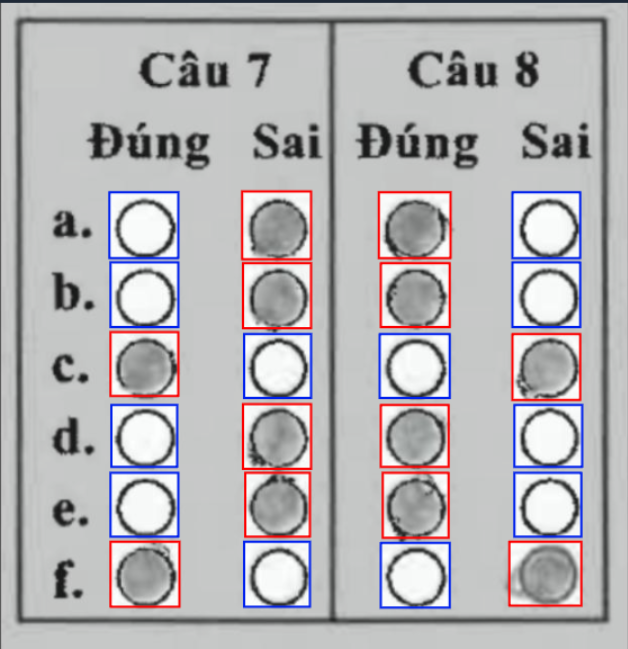
\includegraphics[width=0.85\textwidth]{img_proj/tp2.png}
        \caption{Nhận diện trên phần 2.}
        \label{fig:detection_part2_noise}
    \end{subfigure}
    \hfill
    \begin{subfigure}[b]{0.48\textwidth}
        \centering
        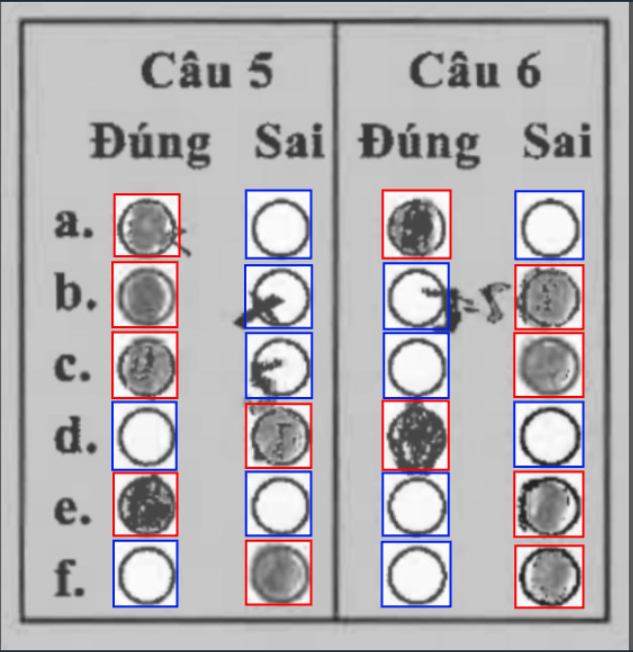
\includegraphics[width=0.85\textwidth]{img_proj/tp22.png}
        \caption{Nhận diện trên phần 2, tô ẩu phức tạp.}
        \label{fig:detection_part2_complex_messy}
    \end{subfigure}
    \caption{Minh họa kết quả nhận diện của mô hình trên các ảnh mẫu.}
    \label{fig:qualitative_detection_examples}
\end{figure}

Từ các ví dụ trực quan (hình \ref{fig:qualitative_detection_examples}), có thể thấy:
\begin{itemize}
    \item Mô hình nhận diện chính xác các ô được tô rõ ràng (Hình \ref{fig:detection_part1_standard}) và vẫn duy trì hiệu suất tốt với các trường hợp tô lem hoặc không đều (hình \ref{fig:detection_part1_messy}).
    \item Mô hình thể hiện khả năng bỏ qua các yếu tố nhiễu như dấu "X" hoặc vết mực nhỏ không phải là hành động tô đáp án (hình \ref{fig:detection_part2_noise}), giúp giảm thiểu dương tính giả.
    \item Ngay cả với các kiểu tô ẩu, phức tạp hoặc có dấu hiệu tẩy xóa, mô hình vẫn cho thấy khả năng phân loại tương đối tốt giữa ô được chọn và không được chọn (hình \ref{fig:detection_part2_complex_messy}).
    \item Nhìn chung, mô hình tỏ ra mạnh mẽ trước sự đa dạng trong cách thí sinh tô đáp án, đây là một yếu tố quan trọng cho ứng dụng thực tế.
\end{itemize}

Các phân tích trực quan này củng cố thêm cho các kết quả định lượng, khẳng định hiệu quả của mô hình trong việc nhận diện các ô được tô trên phiếu trả lời trắc nghiệm.
\section{Chuyển kết quả đầu ra của mô hình thành đáp án lựa chọn}
\label{sec:ung_dung_anh_xa}

Sau khi mô hình nhận diện hiệu quả vị trí của tất cả các ô tròn trên phiếu bài làm, một bước quan trọng tiếp theo là xác định một cách hệ thống xem mỗi ô tròn đó tương ứng với câu hỏi số bao nhiêu và là lựa chọn nào (ví dụ: A, B, C, hay D). Việc này là nền tảng cho quá trình chấm điểm tự động.

\subsection{Trích xuất thông tin vị trí từ mô hình nhận diện}
\label{ssec:trich_xuat_vi_tri}
Mô hình thị giác máy tính đã được huấn luyện có nhiệm vụ quét ảnh phiếu trắc nghiệm và trả về tọa độ các hộp giới hạn (bounding boxes) cho từng ô tròn mà nó phát hiện được. Mỗi hộp giới hạn được định nghĩa bởi tọa độ góc trên bên trái $(x_{\min}, y_{\min})$ và góc dưới bên phải $(x_{\max}, y_{\max})$. Từ các tọa độ này, tọa độ tâm $(x_c, y_c)$ của mỗi ô tròn được tính toán như sau:
\begin{align}
    x_c &= \frac{x_{\min} + x_{\max}}{2} \\
    y_c &= \frac{y_{\min} + y_{\max}}{2}
\end{align}
Tập hợp các tọa độ tâm $(x_c, y_c)$ của tất cả các ô tròn nhận diện được sẽ là đầu vào cho bước xử lý tiếp theo.

\subsection{Ánh xạ lựa chọn bằng phân cụm K-means}
\label{ssec:kmeans_mapping_focused}

Với tập hợp các tọa độ tâm ô tròn, em đề xuất một phương pháp dựa trên thuật toán phân cụm K-means để tổ chức và ánh xạ các ô này vào một cấu trúc lưới logic, phản ánh cách bố trí câu hỏi và lựa chọn trên phiếu. Giả sử vùng đáp án trên phiếu được tổ chức thành $M$ hàng (tương ứng với số câu hỏi hoặc một phần số câu hỏi) và $N$ cột (tương ứng với số lựa chọn cho mỗi câu, ví dụ N=4 cho A, B, C, D). Quá trình này bao gồm các bước sau:

\begin{enumerate}
    \item \textbf{Phân cụm tọa độ X (Xác định cột):}
    Tập hợp các giá trị $x_c$ (hoành độ tâm) của tất cả các ô tròn được đưa vào thuật toán K-means. Số cụm được thiết lập là $K_x = N$ (số lượng lựa chọn cho mỗi câu hỏi). Kết quả của bước này là $N$ tâm cụm theo chiều ngang. Mỗi ô tròn sau đó được gán nhãn cho cột lựa chọn (ví dụ: A, B, C, D) dựa trên việc $x_c$ của nó thuộc về cụm nào. Điều này giúp xác định vị trí tương đối của các cột lựa chọn trên phiếu.

    \item \textbf{Phân cụm tọa độ Y (xác định hàng):}
    Tương tự, tập hợp các giá trị $y_c$ (tung độ tâm) của tất cả các ô tròn được phân cụm bằng K-means với số cụm $K_y = M$ (số lượng hàng câu hỏi trên phiếu hoặc một phần của phiếu). Kết quả là $M$ tâm cụm theo chiều dọc. Mỗi ô tròn được gán nhãn cho hàng câu hỏi tương ứng dựa trên việc $y_c$ của nó thuộc về cụm nào.

    \item \textbf{Tạo lưới logic ánh xạ các ô tô:}
    Sau khi mỗi ô tròn đã được gán một chỉ số hàng (từ phân cụm $y_c$) và một chỉ số cột (từ phân cụm $x_c$), vị trí của nó trong cấu trúc lưới câu hỏi-lựa chọn đã được xác định. Ví dụ, một ô tô có thể được xác định là thuộc "Câu 5, Lựa chọn C". Thông tin này, cùng với tọa độ bounding box gốc, cho phép hệ thống biết chính xác ô tròn nào trên ảnh tương ứng với câu hỏi và lựa chọn nào.
\end{enumerate}

Việc sử dụng K-means cho phép hệ thống linh hoạt với các biến dạng nhỏ hoặc sự xê dịch không đồng đều của các ô tròn trên phiếu, miễn là cấu trúc tổng thể theo hàng và cột vẫn được duy trì tương đối. Số cụm $N$ (số cột/lựa chọn) và $M$ (số hàng/câu hỏi) thường được xác định trước dựa trên cấu trúc chuẩn của mẫu phiếu trắc nghiệm đang được xử lý.

Hình \ref{fig:kmeans_clustering_example_focused} minh họa ý tưởng phân cụm tọa độ tâm các ô tô bằng K-means.
\begin{figure}[H]
    \centering
    % Placeholder cho hình ảnh K-means
        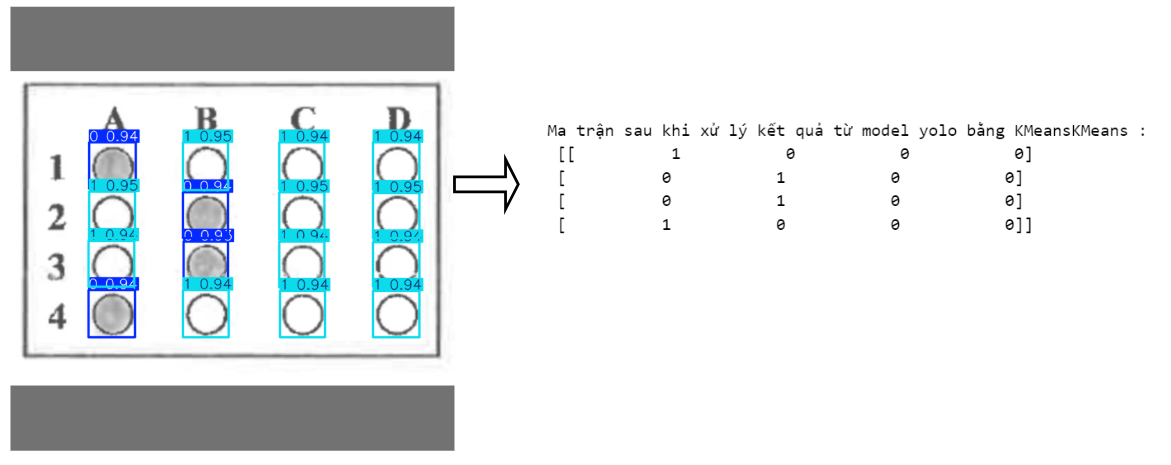
\includegraphics[width=1\textwidth]{img_proj/vd_km.png}
    \caption{Minh họa quá trình phân cụm tọa độ tâm các ô tròn bằng K-means.}
    \label{fig:kmeans_clustering_example_focused}
\end{figure}

Kết quả của quá trình này là một bản đồ chi tiết, liên kết mỗi ô tròn được mô hình nhận diện với một câu hỏi và một lựa chọn cụ thể. Đây là thông tin đầu vào thiết yếu cho các bước tiếp theo trong quy trình chấm điểm, chẳng hạn như xác định ô nào được thí sinh tô chọn và so khớp với đáp án.

\section{Ứng dụng mô hình trong chấm điểm trắc nghiệm}
\label{sec:huong_phat_trien_ung_dung}

Sau quá trình huấn luyện và tinh chỉnh, mô hình nhận diện đối tượng đã đạt được hiệu năng cao trong việc định vị các vùng thông tin quan trọng trên phiếu trả lời trắc nghiệm. Hướng phát triển tiếp theo tập trung vào việc tích hợp mô hình này vào một quy trình chấm điểm tự động hoàn chỉnh.

Cụ thể, thông tin vị trí các ô lựa chọn do mô hình cung cấp sẽ được kết hợp với các thuật toán phân tích trạng thái tô chọn và ánh xạ logic (như đã thảo luận ở mục \ref{ssec:kmeans_mapping_focused} và mục \ref{sec:kien_truc_khoi_nhan_dien_trich_xuat}). Kết quả trích xuất lựa chọn của thí sinh, cùng với thông tin số báo danh và mã đề đã nhận diện, sẽ được đối chiếu tự động với đáp án chuẩn tương ứng.

\begin{figure}[h!]
    \centering
    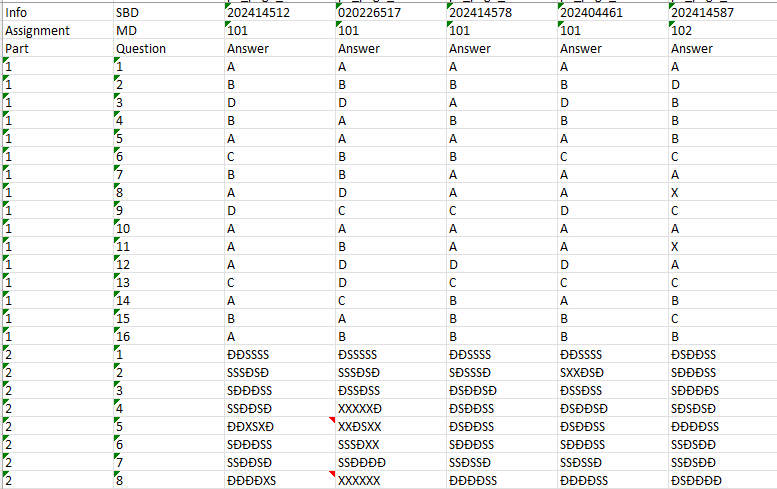
\includegraphics[width=0.85\linewidth]{img_proj/raw.png}
    \caption{Minh họa kết quả thô từ hệ thống}
    \label{fig:enter-label}
\end{figure}

Quy trình này không chỉ cho phép tính toán điểm số một cách nhanh chóng và chính xác mà còn mở ra khả năng tổng hợp và xuất kết quả dưới dạng các tệp tin có cấu trúc, chẳng hạn như bảng tính Excel. Việc này tạo điều kiện thuận lợi cho công tác lưu trữ, quản lý điểm, và phân tích thống kê kết quả thi một cách hiệu quả. Hơn nữa, mô hình có thể được tiếp tục cải tiến và mở rộng để xử lý các loại phiếu trắc nghiệm đa dạng hơn hoặc tích hợp thêm các tính năng nâng cao trong tương lai.








